\documentclass[hidelinks,12pt]{article}
\usepackage[left=0.25cm,top=1cm,right=0.25cm,bottom=1cm]{geometry}
%\usepackage[landscape]{geometry}
\textwidth = 20cm
\hoffset = -1cm
\usepackage[utf8]{inputenc}
\usepackage[spanish,es-tabla, es-lcroman]{babel}
\usepackage[autostyle,spanish=mexican]{csquotes}
\usepackage[tbtags]{amsmath}
\usepackage{nccmath}
\usepackage{amsthm}
\usepackage{amssymb}
\usepackage{mathrsfs}
\usepackage{graphicx}
\usepackage{subfig}
\usepackage{caption}
%\usepackage{subcaption}
\usepackage{standalone}
\usepackage[outdir=./Imagenes/]{epstopdf}
\usepackage{siunitx}
\usepackage{physics}
\usepackage{color}
\usepackage{float}
\usepackage{hyperref}
\usepackage{multicol}
\usepackage{multirow}
%\usepackage{milista}
\usepackage{anyfontsize}
\usepackage{anysize}
%\usepackage{enumerate}
\usepackage[shortlabels]{enumitem}
\usepackage{capt-of}
\usepackage{bm}
\usepackage{mdframed}
\usepackage{relsize}
\usepackage{placeins}
\usepackage{empheq}
\usepackage{cancel}
\usepackage{pdfpages}
\usepackage{wrapfig}
\usepackage[flushleft]{threeparttable}
\usepackage{makecell}
\usepackage{fancyhdr}
\usepackage{tikz}
\usepackage{bigints}
\usepackage{menukeys}
\usepackage{tcolorbox}
\tcbuselibrary{breakable}
\usepackage{scalerel}
\usepackage{pgfplots}
\usepackage{pdflscape}
\pgfplotsset{compat=1.16}
\spanishdecimal{.}
\renewcommand{\baselinestretch}{1.5} 
\renewcommand\labelenumii{\theenumi.{\arabic{enumii}})}

\newcommand{\python}{\texttt{python}}
\newcommand{\textoazul}[1]{\textcolor{blue}{#1}}
\newcommand{\azulfuerte}[1]{\textcolor{blue}{\textbf{#1}}}
\newcommand{\funcionazul}[1]{\textcolor{blue}{\textbf{\texttt{#1}}}}

\newcommand{\pderivada}[1]{\ensuremath{{#1}^{\prime}}}
\newcommand{\sderivada}[1]{\ensuremath{{#1}^{\prime \prime}}}
\newcommand{\tderivada}[1]{\ensuremath{{#1}^{\prime \prime \prime}}}
\newcommand{\nderivada}[2]{\ensuremath{{#1}^{(#2)}}}


\newtheorem{defi}{{\it Definición}}[section]
\newtheorem{teo}{{\it Teorema}}[section]
\newtheorem{ejemplo}{{\it Ejemplo}}[section]
\newtheorem{propiedad}{{\it Propiedad}}[section]
\newtheorem{lema}{{\it Lema}}[section]
\newtheorem{cor}{Corolario}
\newtheorem{ejer}{Ejercicio}[section]

\newlist{milista}{enumerate}{2}
\setlist[milista,1]{label=\arabic*)}
\setlist[milista,2]{label=\arabic{milistai}.\arabic*)}
\newlength{\depthofsumsign}
\setlength{\depthofsumsign}{\depthof{$\sum$}}
\newcommand{\nsum}[1][1.4]{% only for \displaystyle
    \mathop{%
        \raisebox
            {-#1\depthofsumsign+1\depthofsumsign}
            {\scalebox
                {#1}
                {$\displaystyle\sum$}%
            }
    }
}
\def\scaleint#1{\vcenter{\hbox{\scaleto[3ex]{\displaystyle\int}{#1}}}}
\def\scaleoint#1{\vcenter{\hbox{\scaleto[3ex]{\displaystyle\oint}{#1}}}}
\def\scaleiiint#1{\vcenter{\hbox{\scaleto[3ex]{\displaystyle\iiint}{#1}}}}
\def\bs{\mkern-12mu}

\newcommand{\Cancel}[2][black]{{\color{#1}\cancel{\color{black}#2}}}



\author{M. en C. Gustavo Contreras Mayén. \texttt{gux7avo@ciencias.unam.mx}}
\title{Evaluación del Examen Tema 5 - Métodos Monte Carlo \\ {\large Curso Física Computacional}}
\date{ }
\begin{document}

\maketitle
\fontsize{14}{14}\selectfont

\section{Problema 1.}
\begin{enumerate}
\item Al ejecutar el código aparece un error (que no debería) de que no reconoce el \texttt{moduloAleatorio}:
\begin{figure}[H]
    \centering
    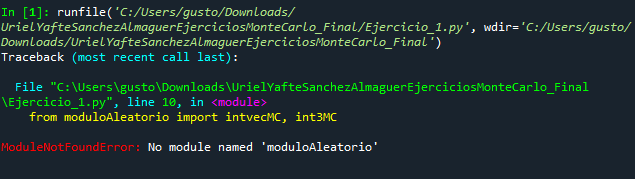
\includegraphics[scale=0.8]{Evidencia_01a.png}
\end{figure}
Se les indicó en la rúbrica que deben de hacer la referencia correspondiente de cada módulo que utilicen.
\item Pasa el mismo error de que no reconoce el \texttt{error\_rel}:
\begin{figure}[H]
    \centering
    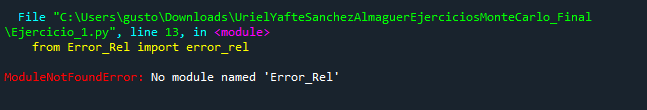
\includegraphics[scale=0.8]{Evidencia_01b.png}
\end{figure}
\item Para que funcione el código en cada inciso del problema, hay que señalar la carpeta donde tienes tu módulo:
\begin{figure}[H]
    \centering
    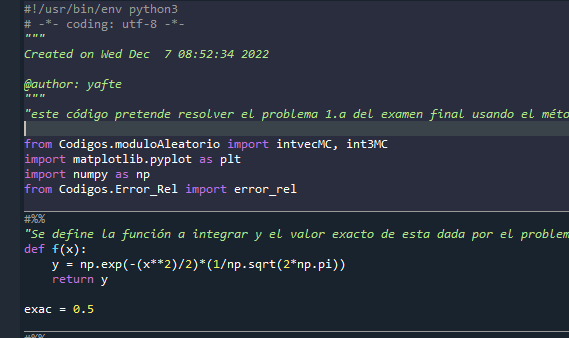
\includegraphics[scale=0.8]{Evidencia_01c.png}
\end{figure}
\item Propones un valor $b = 10000$ como límite superior de integración, que ya de por si es un valor muy grande, considerando el tipo de función que estás manejando, si hubieras graficado inicialmente esa función, hubieras reconocido que no era necesario un valor muy grande.
\begin{figure}[H]
    \centering
    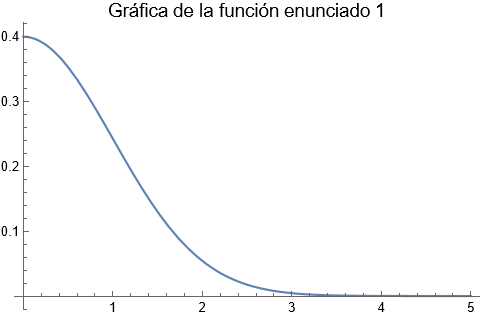
\includegraphics[scale=0.7]{plot_P1_Inciso_01.png}
    \caption{Gráfica para la función del inciso 1 del problema 1.}
\end{figure}
Esta revisión te hubiera simplificado definir el valor para el límite superior de cada integral, mencionas que \enquote{... ya que al usar cantidades más grandes el método MC tiene problemas para mostrar datos que se comporten bien, posiblemente por los recursos computacionales requeridos para calcular la exponencial elevada a términos de orden 1e+10 y superior}, que si bien es cierto, para estos problemas en particular \textbf{no} era necesario definir un valor como el que utilizaste.
\begin{figure}[H]
    \centering
    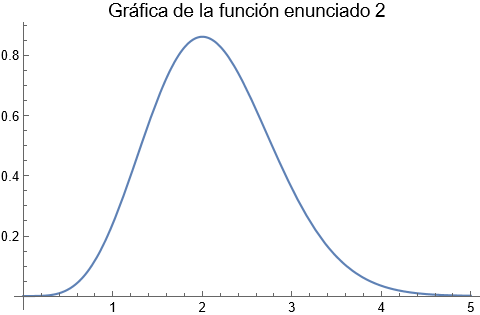
\includegraphics[scale=0.7]{plot_P1_Inciso_02.png}
    \caption{Gráfica para la función del inciso 2 del problema 1.}
\end{figure}
\item El enunciado marca claramente que hagas un cálculo de la integral para diferentes valores de $n$ de $250$ a $\num{d4}$, pero presentas el resultado para el último valor. Se dejó abierta la elección de cuántas evaluaciones se tendrían que hacer, y solo presentas una evaluación.
\item Cuando graficas el valor de la aproximación de la integral y el error relativo, estás mostrando el valor conforme el tamaño de $n$ aumenta y su error asociado, pero el ejercicio pidió que ese contraste se viera con una $n$ pequeña y que fuera cambiando.
\item Como se trabajó en la clase para el método del dardo, se requiere presentar una gráfica para cada valor de $n$ de los puntos aleatorios que están por debajo de la curva y de una cota que se define, no se incluyó esa parte en tu solución.
\item \textbf{Calificación: 0.6 puntos.}
\end{enumerate}

\section{Problema 2.}

\begin{enumerate}
\item Nuevamente al ejecutar el código hay error en las llamadas a las funciones de los módulos. Este detalle penaliza mucho tu ejercicio.
\item Inicias bien con la revisión del problema, es decir, estudias el planteamiento y llegas a una expresión que te permite entonces ocupar las funciones que trabajamos en clase. Es una manera válida que te permite obtener la solución al ejercicio, como comentario, sin ocupar las funciones se puede llegar al mismo resultado, planteando el problema a partir de la geometría: tienes un hemisferio, por geometría puedes trabajar una cuarta parte del mismo y luego encerrarlo en un cubo unitario, para luego con las funciones \texttt{random} expresar la función que define a la esfera y revisar si satisfacen la ecuación de la esfera.
\item Las gráficas iniciales de método de dardo y error relativo los datos se quedan en una columna. ¿Qué pasó?
\item Ahora si incluyes gráficas con los puntos aleatorios por debajo y por arriba de la curva.
\item ¿Por que usaste un valor para $y = 7$? En comparación con el valor de la función queda muy por arriba del valor que si conoces para el hemisferio.
\item En las gráficas que presentas para valores grandes de puntos aleatorio, revisa que tienes una franja de color rojo que son puntos por arriba de la función, pero que están por debajo! 
\item \textbf{Calificación: 0.8}
\end{enumerate}


\end{document}